%% Bookheader, Nov 8, 2020; July 18, 2022

\documentclass[11pt]{../Support/ourbook}
%% or for landscape, comment out line above and use this one:
%%\documentclass[landscape,11pt]{ourbook}

%% This will keep space from stretching around display math:

\makeatletter
\renewcommand\normalsize{%
   \@setfontsize\normalsize\@xipt{13.6}%
   \abovedisplayskip 11\p@  \@minus6\p@
   \abovedisplayshortskip \z@ 
   \belowdisplayshortskip 6.5\p@ \@minus3\p@
   \belowdisplayskip \abovedisplayskip
   \let\@listi\@listI}
\makeatother
\normalsize


\begin{document}

\tableofcontents
\graphicspath{{../../Chapters/volume_double_integral/en_US}}
\chapter{Multiple Integrals}


In this chapter, we extend this powerful idea into higher dimensions using the 
tools of multiple integration. While single integration enables us to calculate
the area under a curve or the volume under a surface, multiple integration 
allows us to calculate volumes in three dimensions, and even hypervolumes in 
higher dimensions.

We start by discussing double integration, which allows us to find the volume 
under a surface in three dimensions. This method involves slicing the solid 
into infinitesimally small columns, and summing the volumes of these columns.

Next, we'll cover triple integration, a tool that lets us find the volume of 
more complicated solids in three-dimensional space. The idea is similar to 
double integration.

To properly implement these techniques, we'll also discuss the different 
coordinate systems that can be used in multiple integration, such as 
rectangular, cylindrical, and spherical coordinates, and when it's advantageous
to use one system over another.

By the end of this chapter, you will have a deeper understanding of the 
techniques of multiple integration and how to apply them to find the volumes 
of various types of solids. The methods we study here will serve as a 
foundation for many topics in higher mathematics and physics, including 
electromagnetism, fluid dynamics, and quantum mechanics.

\section{Double Integrals}
[fixme intro paragraph]

\subsection{Over Rectangular Regions}
Suppose there is some function, $z = f(x,y)$, that is defined over the 
rectangular region, \textit{R}, defined by $\textit{R} = [a, b] \times [c,d] = 
\{(x,y)| a \leq x \leq b, c \leq y \leq d\}$, and $f$ is such that $f \geq 0$ 
for all $(x, y) \in \mathbb{R}$. Then the graph of $f$ is a surface that lies 
above the rectangular region, \textit{R} (see figure \ref{fig:f_on_R}). 

\begin{figure}[htbp]
    \centering
    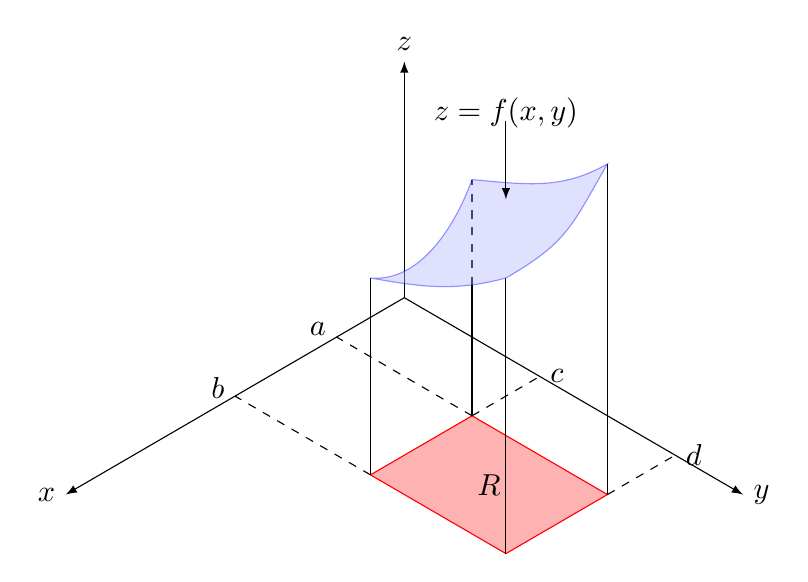
\begin{tikzpicture}[x = {(-0.86cm, -0.5cm)}, y = {(0.86cm, -0.5cm)}, 
    z = {(0cm, 1cm)}]
        \draw[-latex] (0,0,0) -- (5,0,0) node[left] {$x$};
        \draw[-latex] (0,0,0) -- (0,5,0) node[right] {$y$};
        \draw[-latex] (0,0,0) -- (0,0,3) node[above] {$z$};
        \draw[dashed] (1, 2, 0) -- (1, 0, 0) node[left, yshift = 0.1cm] {$a$};
        \draw[dashed] (2.5, 2, 0) -- (2.5, 0, 0) node[left, yshift = 0.1cm] 
        {$b$};
        \draw[dashed] (1, 2, 0) -- (0, 2, 0) node[right] {$c$};
        \draw[dashed] (1, 4, 0) -- (0, 4, 0) node[right] {$d$};
        \filldraw[draw = red, fill = red!30] (1, 2, 0) -- (2.5, 2, 0) -- 
        (2.5, 4, 0) -- (1, 4, 0) -- cycle;
        \node[] at (1.75, 3, 0) {$R$};
        \draw[] (2.5, 2, 0) -- (2.5, 2, 2.5);
        \draw[] (1, 2, 0) -- (1, 2, 1.66);
        \draw[dashed] (1, 2, 1.66) -- (1, 2, 3);
        \draw[] (2.5, 4, 0) -- (2.5, 4, 3.5);
        \draw[] (1, 4, 0) -- (1, 4, 4.2);
        \filldraw[draw = blue, fill = blue!30, opacity = 0.4] (2.5, 2, 2.5) 
        to[out = -5, in = -110, looseness = 0.9] (1, 2, 3) 
        to[out = -5, in = 210] (1, 4, 4.2) 
        to[out = 240, in = 30, looseness = 1.2] (2.5, 4, 3.5) 
        to[out = 195, in = -10] (2.5, 2, 2.5);
        \draw[-latex] (1, 2.5, 4) -- (1, 2.5, 3);
        \node[] at (1, 2.5, 4.1) {$z = f(x,y)$};
    \end{tikzpicture}
    \caption{The graph of $f$ over the region $R$}
    \label{fig:f_on_R}
\end{figure}

Let us call the solid that fills the space between the $xy$-plane and the 
surface $z = f(x,y)$ \textit{S}. Formally, this is written as
$$\textit{S} = \{ (x, y, z) \in \mathbb{R}^3 | 0 \leq z \leq f(x, y), (x, y) 
\in \mathbb{R}\}$$

How can we find the volume of the solid, \textit{S}? We will apply what we 
learned about Riemann sums and definite integrals in two dimensions to this 
three dimensional problem. 

First, we divide \textit{R} into rectangular subregions. We do this by 
dividing the interval $[a, b]$ into \textit{m} subintervals with width $\Delta 
x = (b - a)/m$ and the interval $[c, d]$ into \textit{n} subintervals with 
width $\Delta y = (d - c) / n$. Drawing lines through these divisions parallel 
to the $x$- and $y$-axes, we create a field of subrectangles, each with area 
$\Delta A = \Delta x \Delta y$ (see figure \ref{fig:subrectangles}). Each 
subrectangle is defined by:
$$\textit{R}_{ij} = [x_{i - 1}, x_i] \times [y_{j - 1}, y_j] - \{ (x, y) | x_{
i - 1} \leq x \leq x_i, y_{j - 1} \leq y \leq y_j \}$$ 

\begin{figure}[htbp]
    \centering
    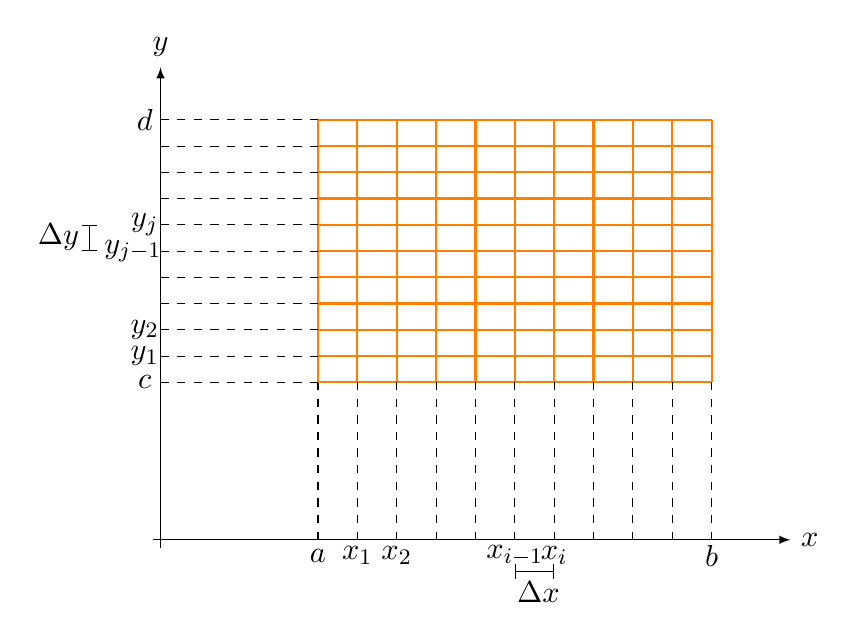
\begin{tikzpicture}
        \draw[-latex] (-0.1, 0) -- (8, 0) node[right] {$x$};
        \draw[-latex] (0, -0.1) -- (0, 6) node[above] {$y$};
        \foreach \i in {0,1, 2, 3, 4, 5, 6, 7, 8, 9, 10} {
            \draw[dashed] (2 + \i/2, 0) -- (2 + \i/2, 2);
            \draw[dashed] (0, 2 + \i/3) -- (2, 2 + \i/3);
            \draw[orange, thick] (2 + \i/2, 2) -- (2 + \i/2, 5.333);
            \draw[orange, thick] (2, 2 + \i/3) -- (7, 2 + \i/3);
            }
        \node[] at (2, -0.2) {$a$};
        \node[] at (7, -0.2) {$b$};
        \node[] at (2.5, -0.2) {$x_1$};
        \node[] at (3, -0.2) {$x_2$};
        \node[] at (4.5, -0.2) {$x_{i - 1}$};
        \node[] at (5, -0.2) {$x_i$};
        \draw[|-|] (4.5, -0.4) -- (5, -0.4) node[below, xshift = -0.2cm] 
        {$\Delta x$};
        \node[] at (-0.2, 2) {$c$};
        \node[] at (-0.2, 5.333) {$d$};
        \node[] at (-0.2, 2.333) {$y_1$};
        \node[] at (-0.2, 2.667) {$y_2$};
        \node[] at (-0.35, 3.667) {$y_{j - 1}$};
        \node[] at (-0.2, 4) {$y_j$};
        \draw[|-|] (-0.9, 3.667) -- (-0.9, 4) node[left, yshift = -0.15cm] 
        {$\Delta y$};
    \end{tikzpicture}
    \caption{The region, \textit{R}, on the $xy$-plane divided into 
    subrectangles}
    \label{fig:subrectangles}
\end{figure}

Since $f(x,y)$ in continuous over the \textit{R}, there is some point, $(x_{ij}
^*, y_{ij}^*)$, equal to the average value of $f(x,y)$ over the subrectangle. 
Then we can approximate the volume between the $xy$-plane and $z = f(x,y)$ over
the subrectangle as a column with base area $\Delta A$ and height $f(x_{ij}^*, 
y_{ij}^*)$ (seefigure \ref{fig:one_column}) and the volume of the column is 
given by:
$$V_{ij} = f(x_{ij}^*, y_{ij}^*) \Delta A$$

\begin{figure}[htbp]
    \centering
    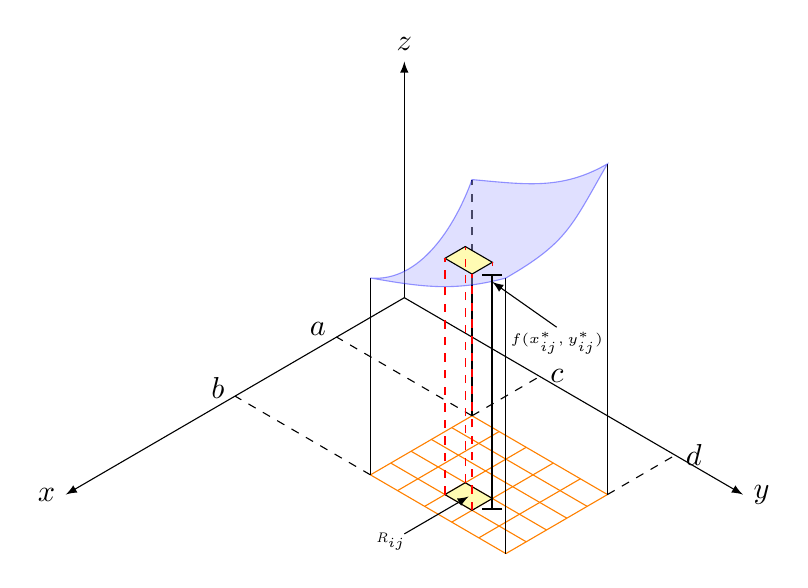
\begin{tikzpicture}[x = {(-0.86cm, -0.5cm)}, y = {(0.86cm, -0.5cm)}, 
    z = {(0cm, 1cm)}]
        \draw[-latex] (0,0,0) -- (5,0,0) node[left] {$x$};
        \draw[-latex] (0,0,0) -- (0,5,0) node[right] {$y$};
        \draw[-latex] (0,0,0) -- (0,0,3) node[above] {$z$};
        \draw[dashed] (1, 2, 0) -- (1, 0, 0) node[left, yshift = 0.1cm] {$a$};
        \draw[dashed] (2.5, 2, 0) -- (2.5, 0, 0) node[left, yshift = 0.1cm] 
        {$b$};
        \draw[dashed] (1, 2, 0) -- (0, 2, 0) node[right] {$c$};
        \draw[dashed] (1, 4, 0) -- (0, 4, 0) node[right] {$d$};
        \foreach \i in {0, 1, 2, 3, 4, 5} {
            \draw[orange] (1 + \i*1.5/5, 2, 0) -- (1 + \i*1.5/5, 4, 0);
            \draw[orange] (1, 2 + 2*\i/5, 0) -- (2.5, 2 + 2*\i/5, 0);
        }
        \draw[] (2.5, 2, 0) -- (2.5, 2, 2.5);
        \draw[] (1, 2, 0) -- (1, 2, 1.66);
        \draw[dashed] (1, 2, 1.66) -- (1, 2, 3);
        \draw[] (2.5, 4, 0) -- (2.5, 4, 3.5);
        \draw[] (1, 4, 0) -- (1, 4, 4.2);
        \filldraw[draw = blue, fill = blue!30, opacity = 0.4] (2.5, 2, 2.5) 
        to[out = -5, in = -110, looseness = 0.9] (1, 2, 3) 
        to[out = -5, in = 210] (1, 4, 4.2) 
        to[out = 240, in = 30, looseness = 1.2] (2.5, 4, 3.5) 
        to[out = 195, in = -10] (2.5, 2, 2.5);
        \filldraw[draw = black, fill = yellow!30] (1.9, 2.8, 0) -- 
        (1.9, 3.2, 0) -- (2.2, 3.2, 0) -- (2.2, 2.8, 0) -- cycle;
        \filldraw[draw = black, fill = yellow!30] (1.9, 2.8, 3) -- 
        (1.9, 3.2, 3) -- (2.2, 3.2, 3) -- (2.2, 2.8, 3) -- cycle;
        \foreach \x/\y in {1.9/2.8, 1.9/3.2, 2.2/3.2, 2.2/2.8} {
            \draw[red, dashed] (\x, \y, 0) -- (\x, \y, 3);
        }
        \draw[|-|, thick] (2.05, 3.35, 0) -- (2.05, 3.35, 3);
        \node[font = \tiny] at (0.75, 3, 1.3) {$f(x_{ij}^*, y_{ij}^*)$};
        \draw[-latex] (0.75, 3, 1.5) -- (2.05, 3.35, 2.9);
        \draw[-latex] (3, 3, 0) -- ( 2.05, 3, 0);
        \node[font = \tiny] at (3.2, 3, 0) {$\textit{R}_{ij}$};
    \end{tikzpicture}
    \caption{A single column with base $\Delta A$ and height $f(x_{ij}^*, 
    y_{ij}^*)$}
    \label{fig:one_column}
\end{figure}

And therefore the approximate volume of the solid, \textit{S}, that lies 
between the region, \textit{R}, and $z = f(x,y)$ is the sum of all the columns 
over $i$ and $j$:
$$V_{\textit{S}} \approx \sum_{i = 1}^n \sum_{j = 1}^n f(x_{ij}^*, y_{ij}^*) 
\Delta A$$

And just like with the area under a curve, we get the true volume by taking the
limit as $n \to \infty$, which becomes a \textbf{double integral}\index{double 
integral}:

\begin{mdframed}[style = important, frametitle = {Volume of a Solid over a 
Region}]
$$V_{\textit{S}} = \lim_{n \to \infty} \sum_{i = 1}^n \sum_{j = 1}^n f(x_{ij}^*
, y_{ij}^*) \Delta A = \iint_{\textit{R}} f(x, y)\,dA$$
\end{mdframed}

Note: a double integral is an integral performed in 2 dimensions at once. It is
not the same as two integrals nested within each other, which we will discuss 
below. 

\section{Iterated Integrals}

To be able to evaluate the double integral as outlined above, we must first 
discuss iterated integrals. Iterated integrals happen when you evaluate two 
single integrals, one inside the other. Consider some function, $g(x, y)$. We 
could integrate that function from $x = q$ to $x = r$ thusly:
$$\int_q^r g(x, y)\,dx$$
Notice that we are integrating with respect to $x$, so $y$ terms will be 
treated as constants (recall partial differentiation: this is the opposite 
process). Let's call the result of this first integral $A(y)$:
$$A(y) = \int_q^r g(x, y)\,dx$$

We can then integrate the resulting function, $A(y)$, from $y = s$ to $y = t$:
$$\int_s^t A(y)\,dy = \int_s^t \left[ \int_q^r g(x, y)\,dx \right]\,dy$$
This is called an \textbf{iterated integral}\index{iterated integral}. When 
evaluating iterated integrals, we work from the inside out. You can also write 
it without the brackets:
$$\int_s^t \int_q^r g(x, y)\,dx\,dy$$

\textbf{Example}: evaluate the iterated integral $\int_0^3 \int_1^2 x y^2\,dy
\,dx$.

\textbf{Solution}: We can re-write this to more explicitly show the inner and 
outer integrals:
$$\int_0^3 \left[ \int_1^2 x y^2\,dy \right]\,dx$$
As you can see, the inner integral is with respect to $y$. Let's isolate and 
evaluate the inner integral:
$$\int_1^2 x y^2\,dy = x \int_1^2 y^2\,dy = x \left[ \frac{1}{3}y^2 \right]_{y 
= 1}^{y = 2}$$
$$= \frac{x}{3} \left[ 2^3 - 1^3 \right] = \frac{x}{3} \left[ 8 - 1 \right] = 
\frac{7x}{3}$$

We were able to move $x$ outside the integral because when we are integrating 
with respect to a specific variable (in this case, $y$), other variables are 
treated as constants. Now we can substitute $\int_1^2 xy^2 \,dy = \frac{7x}{3}$
into the iterated integral:
$$\int_0^3 \left[ \int_1^2 x y^2\,dy \right]\,dx = \int_0^3 \left[ \frac{7x}{3}
\right]\,dx$$
$$= \frac{7}{3} \left[ \frac{1}{2}x^2 \right]_{x = 0}^{x = 3} = \frac{7}{6} 
\left[ 3^2 - 0^2 \right] = \frac{7 \cdot 9}{6} = \frac{21}{2}$$

\begin{Exercise}[title = {Order of Evaluating Iterated Integrals}, label = 
iterate 1]
Show that $\int_0^3 \int_1^2 x y^2\,dy\,dx = \int_1^2 \int_0^3 x y^2 \,dx\,dy$.
\end{Exercise}

\begin{Answer}[ref = iterate_1]
We have already shown that $\int_0^3 \int_1^2 x y^2\,dy\,dx = \frac{21}{2}$. 
We will evaluate $\int_1^2 \int_0^3 x y^2 \,dx\,dy$ and see if we get the same 
result. 
$$\int_0^3 x y^2 \,dx = y^2 \int_0^3 x\,dx = y^2 \left[ \frac{1}{2}x^2 \right]_
{x = 0}^{x = 3}$$
$$= \frac{y^2}{2} \left[ 3^2 - 0^2 \right] = \frac{9y^2}{2}$$
Substituting this back into the iterated integral:
$$\int_1^2 \int_0^3 x y^2 \,dx\,dy = \int_1^2 \frac{9y^2}{2}\,dy = \frac{9}{2} 
\int_1^2 y^2 \,dy$$
$$= \frac{9}{2} \left[ \frac{1}{3}y^3 \right]_{y = 1}^{y = 2} = \frac{9}{2} 
\cdot \frac{1}{3} \left[ 2^3 - 1^3 \right]$$
$$= \frac{3}{2}(8 - 1) = \frac{21}{2}$$
\end{Answer}

\begin{Exercise}[title = {Evaluating Iterated Integrals}, label = iterate_2]
Evaluate the following iterated integrals.
\begin{enumerate}
\item $\int_0^1 \int_1^2 \left( x + e^{-y} \right)\,dx\,dy$
\item $\int_{-3}^3 \int_{0}^{\pi/2} \left( 2y + y^2 \cos{x} \right)\,dx\,dy$
\item $\int_0^3 \int_0^{\pi/2} t^2 \sin^3{\theta}\,d\theta\,dt$
\end{enumerate}
\vspace{100mm}
\end{Exercise}

\begin{Answer}[ref = iterate_2]
\begin{enumerate}
\item Answer: $\frac{5}{2} - \frac{1}{e}$. Solution: $\int_0^1 \int_1^2 \left( 
x + e^{-y} \right)\,dx\,dy = \int_0^1 \left( \frac{1}{2}x^2 + xe^{-y} \right)
|_{x=1}^{x=2}\,dy = \int_0^1 \left( 2 - \frac{1}{2} + 2e^{-y} - e^{-y} \right)
\,dy = \int_0^1 \left( \frac{3}{2} + e^{-y} \right)\,dy = \left[ \frac{3}{2}y 
- e^{-y} \right]_{y = 0}^{y = 1} = \left( \frac{3}{2}(1) - e^{-1} \right) - 
\left( \frac{3}{2}(0) - e^0 \right) = \frac{5}{2} - \frac{1}{e}$
\item Answer: $18$. Solution: $\int_{-3}^3 \int_{0}^{\pi/2} \left( 2y + y^2 
\cos{x} \right)\,dx\,dy = \int_{-3}^3 \left[ 2xy + y^2 \sin{x} \right]_{x = 0}^
{x = \pi/2}\,dy = \int_{-3}^3 \left[ \left( \pi y + y^2 \right) - \left( 0 + 0 
\right) \right]\,dy = \int_{-3}^3 \left( \pi y + y^2 \right)\,dy = \left[ 
\frac{\pi}{2}y^2 + \frac{1}{3}y^3 \right]_{y = -3}^{y = 3} = \left( \frac{\pi}{
2}(9) + \frac{1}{3}(27) \right) - \left( \frac{\pi}{2}(9) + \frac{1}{3}(-27) 
\right) = 9 - (-9) = 18$
\item Answer: $6$. Solution: $\int_0^3 \int_0^{\pi/2} t^2 \sin^3{\theta}\,
d\theta\,dt = \left( \int_0^3 t^2\,dt \right) \times \left( \int_0^{\pi/2} 
\sin^3{\theta}\,d\theta \right) = \left[ \frac{1}{3}t^3 \right]_{t = 0}^{t = 3}
\times \left( \int_0^{\pi/2} \sin{\theta} \sin^2{\theta}\,d\theta \right) = 9
\int_0^{\pi/2} \sin{\theta} \left( 1 - \cos^2{\theta} \right)\,d\theta = 9 
\left[ \int_0^{\pi/2} \sin{\theta}\,d\theta - \int_0^{\pi/2} \sin{\theta}
\cos^2{\theta}\,d\theta \right] = 9 \left[ \left( -\cos{\theta} \right) |_{
\theta = 0}^{\theta = \pi/2} + \left( \frac{1}{3}\cos^3{\theta} \right)|_{
\theta = 0}^{\theta = \pi/2} \right] = 9 \left[ -(-\cos{0}) + (-\frac{1}{3}
\cos^3{0}) \right] = 9 \left( 1 - \frac{1}{3} \right) = 9 \left( \frac{2}{3} 
\right) = 6$
\end{enumerate}
\end{Answer}

\section{Fubini's Theorem for Double Integrals}

\begin{mdframed}[style = important, frametitle = {Fubini's Theorem}]
If $f$ is continuous on the rectangle $R = \{ \left( x, y \right) | a \leq x 
\leq b, c \leq y \leq d \}$, then
$$\iint_R f(x,y)\,\,dA = \int_a^b \int_c^d f(x,y)\,dy\,dx = \int_c^d \int_a^b 
f(x,y)\,dx\,dy$$
\end{mdframed}

\begin{Exercise}[title={Applying Fubini's Theorem},label = fubini]
Rewrite the following double integrals as iterated integrals.
\begin{enumerate}
\item $\iint_R \frac{xy^2}{x^2 + 1}\,\,dA$, $R = \{(x,y)|0 \leq x \leq 1, -3 
\leq y \leq 3\}$
\item $\iint_R \frac{\sec{\theta}}{\sqrt{1 + t^2}}\,\,dA$, $R = \{(\theta, t) |
0 \leq \theta \leq \frac{\pi}{4}, 0 \leq t \leq 1 \}$
\end{enumerate}
\vspace{40mm}
\end{Exercise}

\begin{Answer}[ref = fubini]
\begin{enumerate}
\item $\int_0^1 \int_{-3}^3 \frac{xy^2}{x^2 + 1}\,dy\,dx$ OR $\int_{-3}^3 
\int_0^1 \frac{xy^2}{x^2 + 1}\,dx\,dy$
\item $\int_0^{\pi/4} \int_0^1 \frac{\sec{\theta}}{\sqrt{1 + t^2}}\,dt\,
d\theta$ OR $\int_0^1 \int_0^{\pi/4} \frac{\sec{\theta}}{\sqrt{1 + t^2}}\,
d\theta \,dt$
\end{enumerate}
\end{Answer}

\begin{Exercise}[title={Using Polar Coordinates in Multiple Integration}, 
label=polarmulti]

\Question Use double integration to find the volume of the solid that lies under the surface $z = 4 - x^2 - y^2$ and above the $xy$-plane.

\end{Exercise}
\begin{Answer}[ref=polarmulti]

We are finding the volume of the solid that lies under the surface $z = 4 - x^2 - y^2$ and above the $xy$-plane.

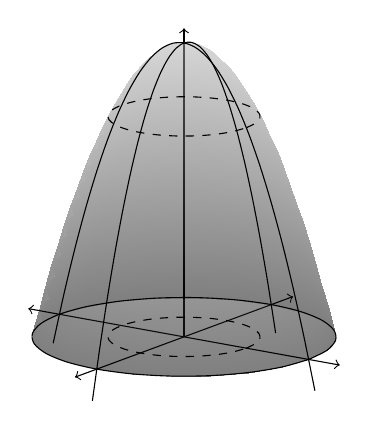
\begin{tikzpicture}
  \begin{axis}[
    view={35}{15},
    unit vector ratio=1 1 1,
    ticks = none,
    axis lines=middle,
    ymin=-2.5,
    ymax=2.5,
    xmax=2.5,
    xmin=-2.5,
    zmin=0,
    zmax=4.2,
    x axis line style=<->,
    y axis line style=<->,
    z axis line style=->,
    clip=false
  ]
    \addplot3[surf,shader=interp,domain=0:360,y domain=0:2, opacity=0.5,
    colormap={blackwhite}{color=(black) color=(black!30)}] ({y*cos(x)},
    {y*sin(x)},{4-y^2});
    \addplot3[samples y=0,domain=0:360,smooth]({2*cos(x)},  {2*sin(x)},0);
    \addplot3[samples y=0,domain=0:360,smooth,dashed]({cos(x)},  {sin(x)},0);
    \addplot3[samples y=0,domain=0:360,smooth,dashed]({cos(x)},  {sin(x)},3);
    \addplot3[samples y=0,domain=-2.1:2.1,smooth](0,  {x},{4 - x^2});
    \addplot3[samples y=0,domain=-2.1:2.1,smooth]({x},0, {4 - x^2});
  \end{axis}
\end{tikzpicture}

We can use polar coordinates to simplify the double integral. In polar coordinates, $x = r\cos(\theta)$ and $y = r\sin(\theta)$, so $x^2 + y^2 = r^2$. The volume under the surface and above the $xy$-plane is given by

\begin{equation}
V = \int \int (4 - r^2) r \, dr \, d\theta,
\end{equation}

where $r$ ranges from 0 to 2 (since $4 - r^2 \geq 0$ if $0 \leq r \leq 2$) and $\theta$ ranges from 0 to $2\pi$.

Hence,

\begin{align*}
V & = \int_{0}^{2\pi} \int_{0}^{2} (4r - r^3) \, dr \, d\theta \\
& = \int_{0}^{2\pi} \left[ 2r^2 - \frac{1}{4}r^4 \right]_{0}^{2} \, d\theta \\
& = \int_{0}^{2\pi} (8 - 4) \, d\theta \\
& = \int_{0}^{2\pi} 4 \, d\theta \\
& = \left[ 4\theta \right]_{0}^{2\pi} \\
& = 8\pi.
\end{align*}

So the volume of the solid is $8\pi$ cubic units.

\end{Answer}

\section{Triple Integrals}

\graphicspath{{../../Chapters/multiv_dist/en_US}}
\chapter{Multivariate Distributions}

The world of probability and statistics doesn't limit itself to the
study of single variables. Often, we are interested in the
interconnections, relationships, and associations among several
variables. In such a scenario, the univariate distributions that we
have studied so far become inadequate. To comprehend the joint
behavior of these variables and to uncover the underlying patterns of
dependency, we must turn to the realm of multivariate distributions.

This chapter aims to introduce the reader to the concept of
multivariate probability distributions. These are probability
distributions that take into account and describe the behavior of more
than one random variable. We will start our exploration with a
discussion on the joint probability mass and density functions. These
functions extend the concepts of probability mass and density
functions for one variable to the situation where we have multiple
variables.

Next, we will explore important properties of joint distributions,
including the concept of marginal distribution and conditional
distribution, which allow us to explore the probability of a subset of
variables while conditioning on, or ignoring, other variables. We will
also introduce the idea of independence of random variables in the
multivariate context.

Subsequently, we will discuss some commonly used multivariate
distributions such as the multivariate normal distribution, and the
multivariate Bernoulli and binomial distributions. These specific
distributions will provide us with practical tools for modelling
multivariate data.

Finally, we will delve into covariance and correlation, two key
measures that give us a sense of how two variables change
together. Understanding these measures is critical for capturing the
relationships in multivariate data.



\graphicspath{{../../Chapters/multiv_normal/en_US}}
\chapter{The Multivariate Normal Distribution}

Let's say that you are gathering statistics on a species of snail. You have found 89 snails.
Every snail has been weighted and had its shell measured. You have created a table like this:

\begin{tabular}{ c c }
Weight & Diameter \\
\hline
4.4769 grams & 2.2692 cm\\
5.4755 grams & 2.1973 cm\\
4.1183 grams & 2.52928 cm\\
... & ... \\
3.0522 grams & 1.7822 cm
\end{tabular}


You have been told that for any particular species of snail, the weight and shell diameter are typically normally distributed.
So, you compute the mean of each:

$$\bar{x} = \frac{\sum_{i=1}^{n} x_i}{n}$$

Your snails have a mean mass off 4.25 grams and a mean shell diameter of 2.35 centimeters.
Now you know where the center of each normal distribution will be.

To know how wide each normal distribution is, you need to compute the variance:

$$\sigma^2 = \frac{\sum_{i=1}^{n} (x_i - \bar{x})^2}{n}$$

(Reminder: The standard deviation is the square root of $\sigma^2$)

Plotting this data is shown in Figure~\ref{fig:pdfweight_diameter}.
\begin{figure}[htbp]
    \centering
    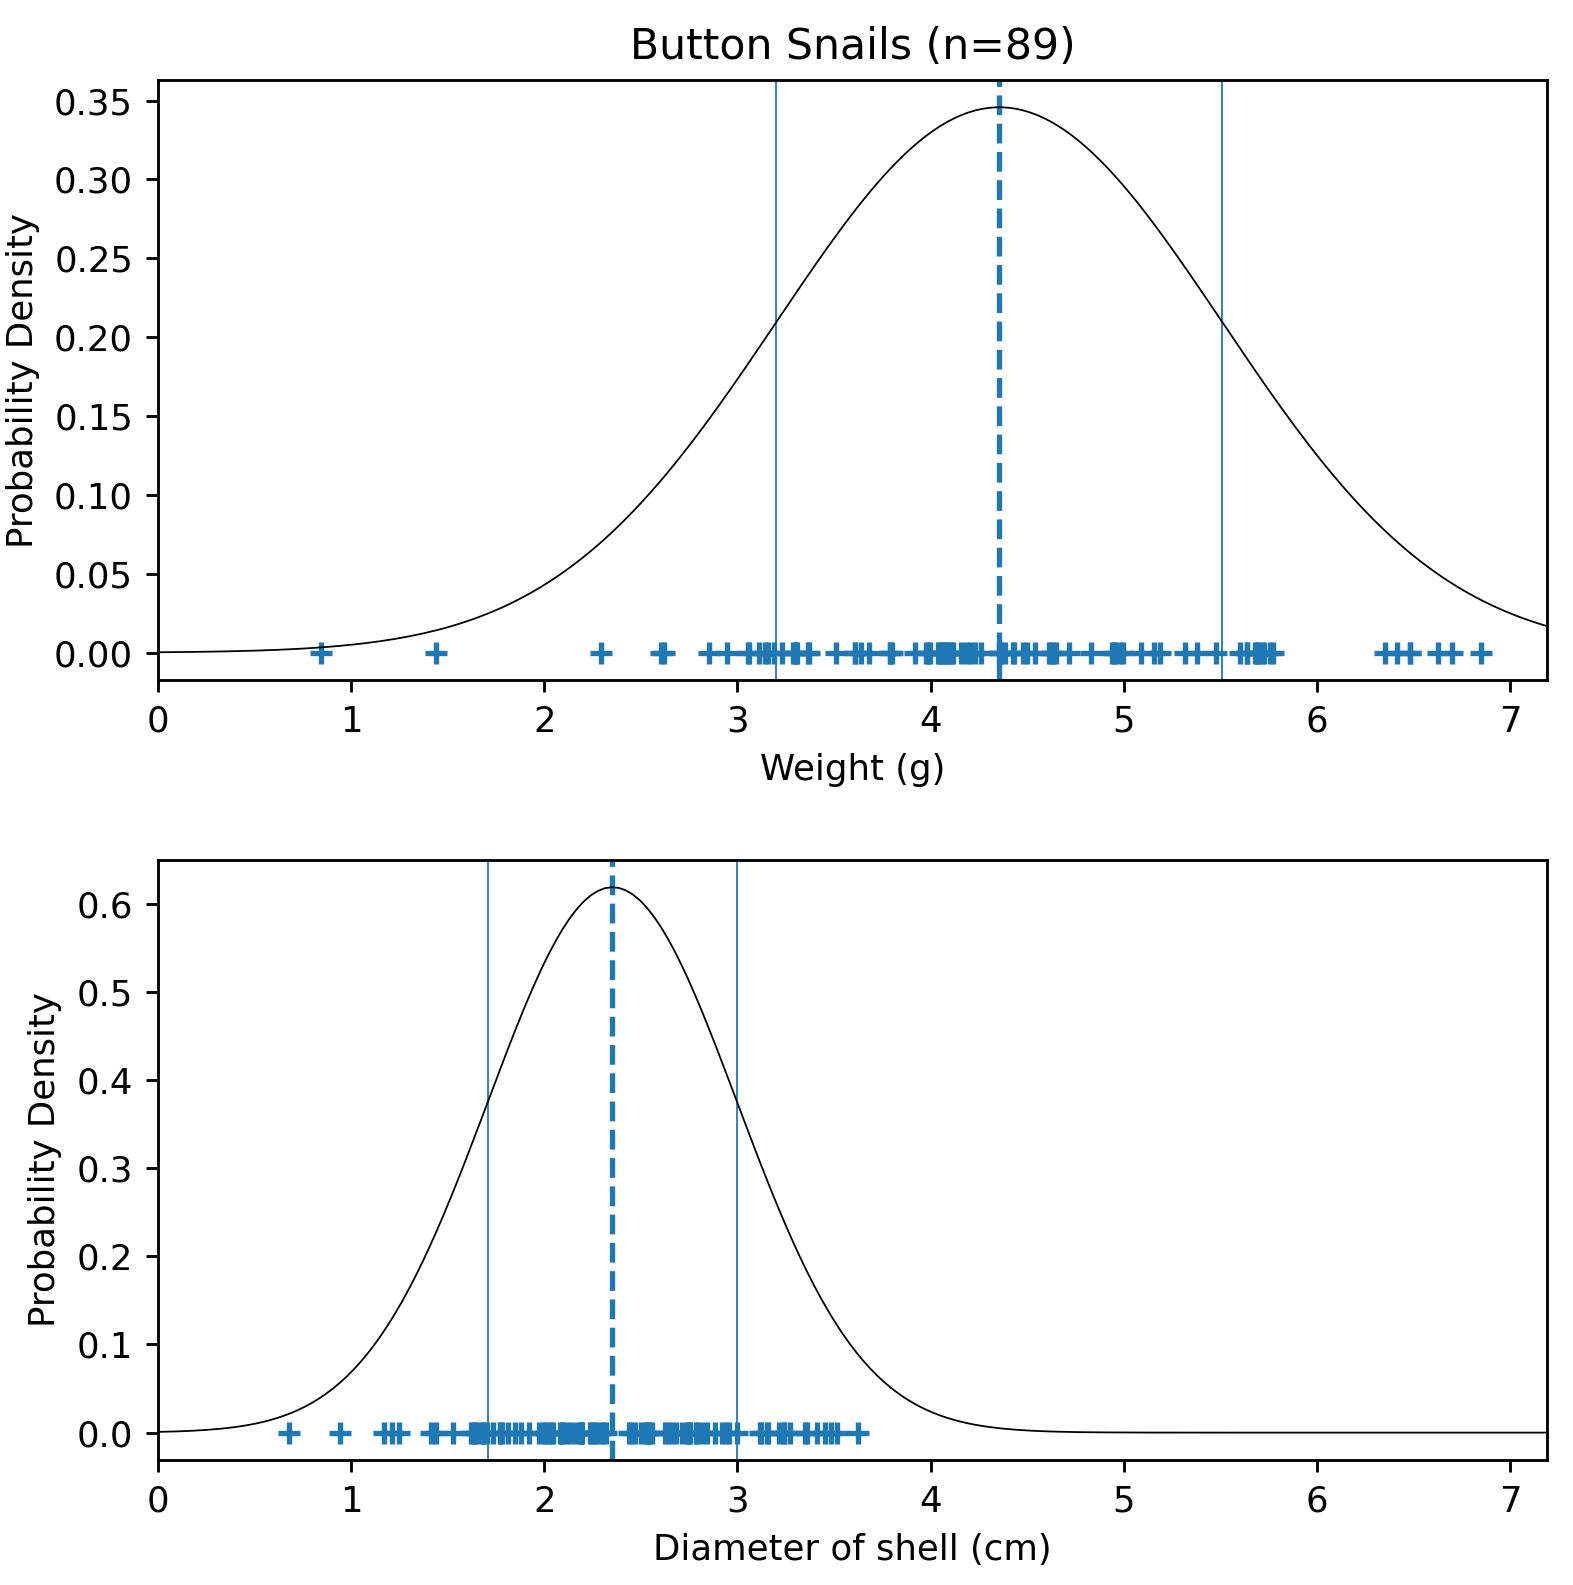
\includegraphics[width=0.55\textwidth]{separate.png}
    \caption{Probability density functions of weight and diameter.}
    \label{fig:pdfweight_diameter}
\end{figure}

Nice! However, then you think: "Hmm. Maybe the mass and the diameter of the shell are related. It seems like a heavy snail might tend to have a larger shell."  So, you make a scatter plot:

\begin{figure}[htbp]
    \centering
    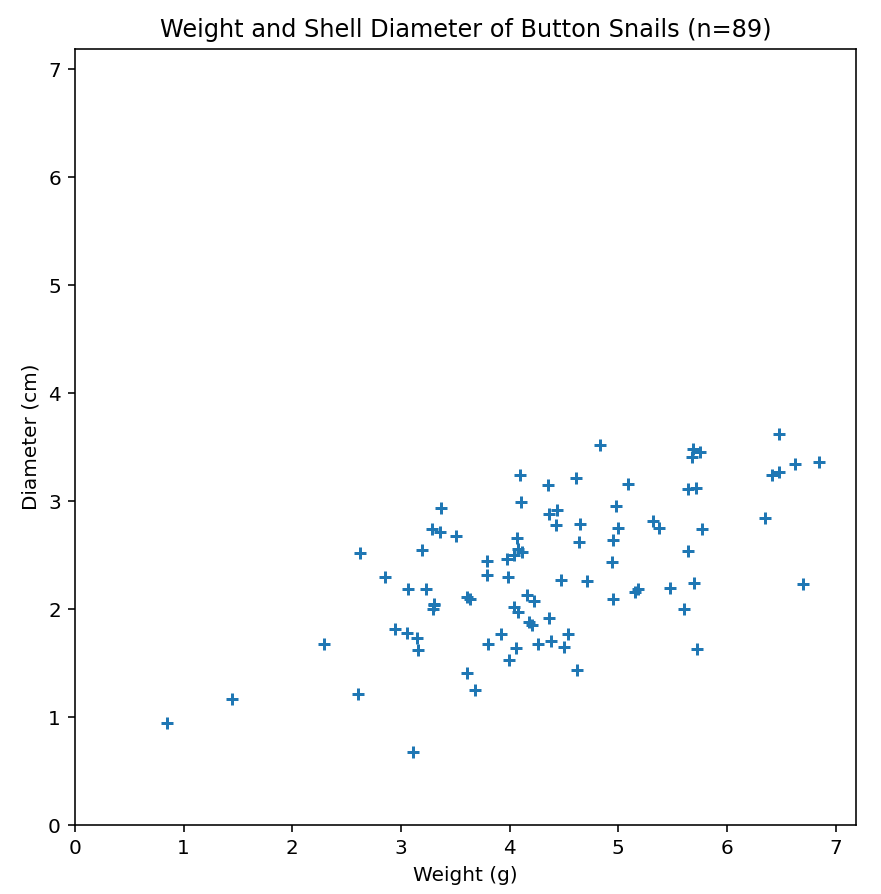
\includegraphics[width=0.55\textwidth]{scatter.png}
    \caption{A scatter plot with weight of the snail horizontally and diamter of the shell on the y-axis.}
    \label{fig:example}
\end{figure}

Sure enough, there is some correlation between the mass of the snail and the diameter of its shell.

There is a form of the normal distribution that can deal with multiple variables and their correlations.
This is known as the \newterm{multivariate normal} or the \newterm{Gaussian distribution}. \index{multivariate normal distribution} \index{Gaussian distribution}

In a multivariate normal distribution, the mean (often denoted $\boldsymbol\mu$) is a vector containing the mean of every variable.
For your snails, $\boldsymbol\mu = \begin{bmatrix} 4.25, 2.35 \end{bmatrix}$.

Just as in the single-variable normal distribution, measurements near the mean are what you are most likely to observe.
In a single-variable normal distribution, the standard deviation tells us how fast that likelihood falls off as we move away from the mean.
In multivariate normal distributions, we need something a little more expressive: a matrix.

\section{The Covariance Matrix}

We can think of the data as a list of vectors.
For example, if we have $n$ snails and $d$ properties that we have measured, we would get a list like this:

$$\begin{bmatrix}
x_{1,1} & x_{1,2} & ... & x_{1,d} \\
x_{2,1} & x_{2,2} & ... & x_{2,d} \\
... & ... & &... \\
x_{n,1} & x_{n,2} & ... & x_{b,d}\end{bmatrix}$$

Each row represents one snail. Each column represents one property.

Note that to make $\boldsymbol\mu$ (the mean vector), you just take the mean of each column of this data matrix. (For convenience, we will use $\boldsymbol\mu_i$ to refer to the mean of column $i$.)

We usually use $\mathbf{\Sigma}$ (the uppercase Greek sigma) to represent a covariance matrix. $\mathbf{\Sigma}$ is a $d \times d$ matrix.
The entries on the diagonal of $\mathbf{\Sigma}$ are just the variance of each property.
So, we can caluculate the entry at row $j$, column $j$ like this:

$$\mathbf{\Sigma}_{j,j} = \frac{\sum_{i=1}^{n}(x_{i,j} - \boldsymbol\mu_j)^2}{n}$$

(Yes, we are using $\mathbf{\Sigma}$ to represent both summation and the covariance matrix here.
It can be confusing, but you will be able to tell from context how it is being used.)

The other entries, $\Sigma_{j,k}$ where $j \neq k$, are the \newterm{covariance} between property $j$ and property $k$.
If the covariance is a positive number, property $j$ and property $k$ are correlated. For example, in your snails, weight and diameter have a positive covariance: If the snail is heavier than average, it tends to have a diameter that is larger than average.

If the covariance is a negative number, when property $j$ is greater than average, property $k$ tends to be less than average.
For example, the number of times a restaurant mops the floor in a week has a negative covariance with how much bacteria lives on the floor.

How do we compute the covariance?

$$\mathbf{\Sigma}_{j,k} = \frac{\sum_{i=1}^{n}(x_{i,j} - \boldsymbol\mu_j)(x_{i,k} - \boldsymbol\mu_k)}{n}$$

Note that $\mathbf{\Sigma}_{j,k} = \mathbf{\Sigma}_{k,j}$, so the matrix is symmetric.

\subsection{Computing Mean and Covariance in Python}

If you have a numpy array where each row represents one sample and each column represents one property, it is really easy to compute $\boldsymbol\mu$ and $\mathbf{\Sigma}$:

\begin{verbatim}
# Read in the data matrix, each row represents one snail
snails = ...

# Compute mu
mean_vector = snails.mean(axis=0)
print(f"Mean = {mean_vector}")

# Compute Sigma
covariance_matrix = np.cov(snails, rowvar=False)
print(f"Covariance = {covariance_matrix}")
\end{verbatim}

\section{Multivariate Normal Probability Density}

Now that we have good estimates of $\boldsymbol\mu$ and $\mathbf{\Sigma}$, how can we compute the probability density?

When you were working with just one variable, $x$, you computed the probability density using the mean $\mu$ and the variance $\sigma^2$ like this:

\begin{equation*}
p(x) = \frac{1}{\sqrt{2\pi\sigma^2}} e^{-\frac{(x - \mu)^2}{2\sigma^2}}
\end{equation*}

The probability density function of a $d$-dimensional
multivariate normal distribution with a mean of $\boldsymbol\mu$ and a covariance matrix of $\mathbf{\Sigma}$ is given by:

\begin{equation*}
p(\mathbf{x}) = \frac{1}{\sqrt{(2\pi)^d|\mathbf{\Sigma}|}}\exp\left(-\frac{1}{2}(\mathbf{x}-\boldsymbol\mu)^T\mathbf{\Sigma}^{-1}(\mathbf{x}-\boldsymbol\mu)\right)
\end{equation*}

If we draw lines to show where $\boldsymbol\mu$ is and contours to show lines of equal probability density, we get a plot shown in Figure~\ref{fig:contour_snail}.
\begin{figure}[htbp]
    \centering
    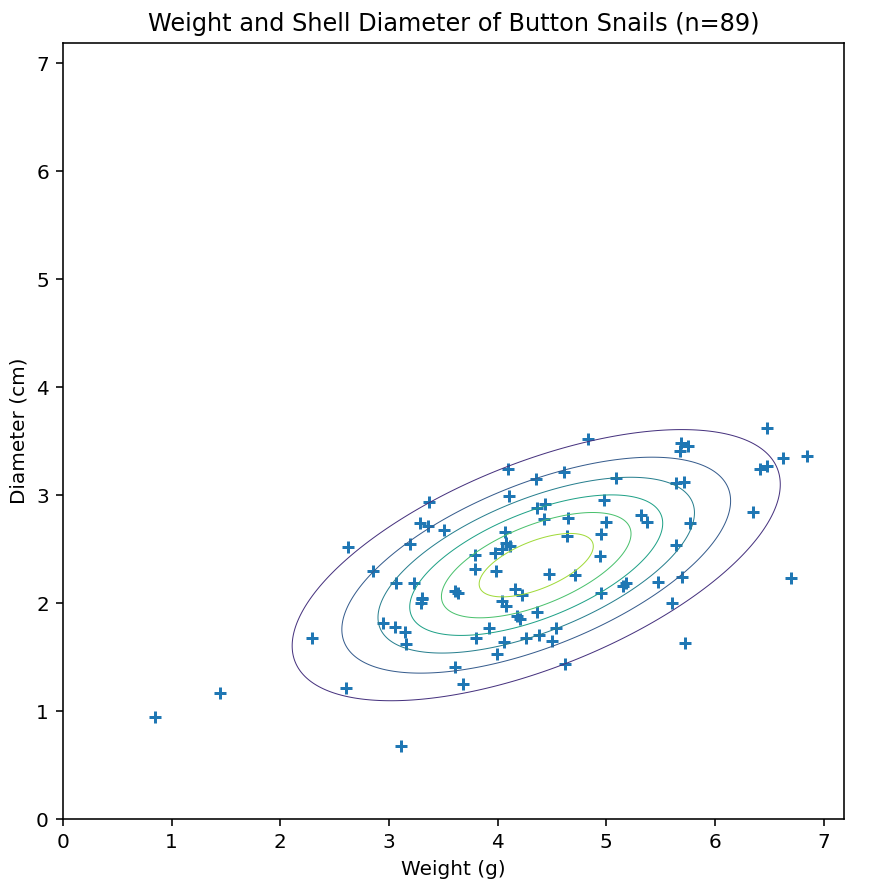
\includegraphics[width=0.55\textwidth]{contour.png}
    \caption{Contour plot of the snail data.}
    \label{fig:contour_snail}
\end{figure}

Or, we can do a 3D plot, as shown in Figure~\ref{fig:3d_snail}.
\begin{figure}[htbp]
    \centering
    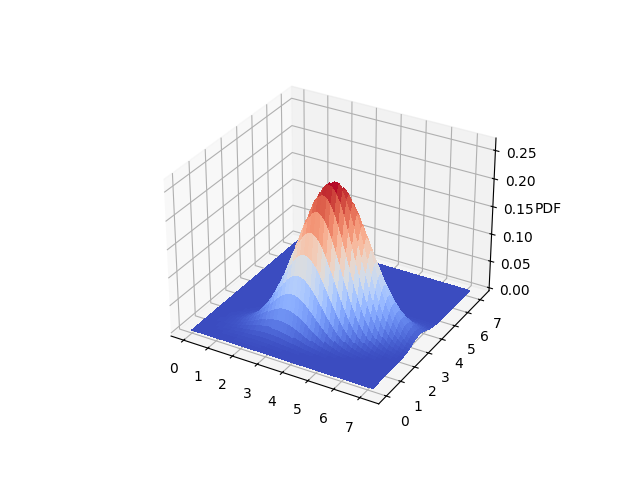
\includegraphics[width=0.55\textwidth]{3d.png}
    \caption{3D plot of the probability density function.}
    \label{fig:3d_snail}
\end{figure}

A probability density always integrates to 1.0, so the volume under the surface must be 1.0.

\subsection{Multivariate Normal Probability Density in Python}

The scipy library has a class that represents the multivariate normal. Here is how you could compute the probability density for a particular snail:

\begin{verbatim}
import numpy as np
from scipy.stats import multivariate_normal

...Compute mean_vector and covariance_matrix...

# Get the probability density at [3 grams, 2 cm]
x = np.array([3.0, 2.0])
pd = multivariate_normal.pdf(x, mean=mean_vector, cov=covariance_matrix)
print(f"The probability density at {x} is {pd}")
\end{verbatim}

Alternatively, maybe you would like to generate weights and diameters for a fictional population of 700 snails:

\begin{verbatim}
new_snails = multivariate_normal.rvs(mean=mean_vector, cov=covariance_matrix, size=700)
print(f"My fictional snails:\n{new_snails}")
\end{verbatim}

%%%%%%%%%%%%%%%%%%%%%%%%%%%%%%%%%
%% Bookfooter.tex by Aaron Hillegass
%% Nov 8, 2020

\appendix

\chapter{Answers to Exercises}
\shipoutAnswer

\bibliography{references}

\printindex

\end{document}